\documentclass[11pt,a4paper,]{article}
\usepackage{lmodern}

\usepackage{amssymb,amsmath}
\usepackage{ifxetex,ifluatex}
\usepackage{fixltx2e} % provides \textsubscript
\ifnum 0\ifxetex 1\fi\ifluatex 1\fi=0 % if pdftex
  \usepackage[T1]{fontenc}
  \usepackage[utf8]{inputenc}
\else % if luatex or xelatex
  \usepackage{unicode-math}
  \defaultfontfeatures{Ligatures=TeX,Scale=MatchLowercase}
\fi
% use upquote if available, for straight quotes in verbatim environments
\IfFileExists{upquote.sty}{\usepackage{upquote}}{}
% use microtype if available
\IfFileExists{microtype.sty}{%
\usepackage[]{microtype}
\UseMicrotypeSet[protrusion]{basicmath} % disable protrusion for tt fonts
}{}
\PassOptionsToPackage{hyphens}{url} % url is loaded by hyperref
\usepackage[unicode=true]{hyperref}
\hypersetup{
            pdftitle={The Causes of Death around the World},
            pdfborder={0 0 0},
            breaklinks=true}
\urlstyle{same}  % don't use monospace font for urls
\usepackage{geometry}
\geometry{a4paper, centering, text={16cm,24cm}}
\usepackage[style=authoryear-comp,]{biblatex}
\addbibresource{references.bib}
\usepackage{longtable,booktabs}
% Fix footnotes in tables (requires footnote package)
\IfFileExists{footnote.sty}{\usepackage{footnote}\makesavenoteenv{long table}}{}
\usepackage{graphicx,grffile}
\makeatletter
\def\maxwidth{\ifdim\Gin@nat@width>\linewidth\linewidth\else\Gin@nat@width\fi}
\def\maxheight{\ifdim\Gin@nat@height>\textheight\textheight\else\Gin@nat@height\fi}
\makeatother
% Scale images if necessary, so that they will not overflow the page
% margins by default, and it is still possible to overwrite the defaults
% using explicit options in \includegraphics[width, height, ...]{}
\setkeys{Gin}{width=\maxwidth,height=\maxheight,keepaspectratio}
\IfFileExists{parskip.sty}{%
\usepackage{parskip}
}{% else
\setlength{\parindent}{0pt}
\setlength{\parskip}{6pt plus 2pt minus 1pt}
}
\setlength{\emergencystretch}{3em}  % prevent overfull lines
\providecommand{\tightlist}{%
  \setlength{\itemsep}{0pt}\setlength{\parskip}{0pt}}
\setcounter{secnumdepth}{5}

% set default figure placement to htbp
\makeatletter
\def\fps@figure{htbp}
\makeatother


\title{The Causes of Death around the World}

%% MONASH STUFF

%% CAPTIONS
\RequirePackage{caption}
\DeclareCaptionStyle{italic}[justification=centering]
 {labelfont={bf},textfont={it},labelsep=colon}
\captionsetup[figure]{style=italic,format=hang,singlelinecheck=true}
\captionsetup[table]{style=italic,format=hang,singlelinecheck=true}


%% FONT
\RequirePackage{bera}
\RequirePackage[charter,expert,sfscaled]{mathdesign}
\RequirePackage{fontawesome}

%% HEADERS AND FOOTERS
\RequirePackage{fancyhdr}
\pagestyle{fancy}
\rfoot{\Large\sffamily\raisebox{-0.1cm}{\textbf{\thepage}}}
\makeatletter
\lhead{\textsf{\expandafter{\@title}}}
\makeatother
\rhead{}
\cfoot{}
\setlength{\headheight}{15pt}
\renewcommand{\headrulewidth}{0.4pt}
\renewcommand{\footrulewidth}{0.4pt}
\fancypagestyle{plain}{%
\fancyhf{} % clear all header and footer fields
\fancyfoot[C]{\sffamily\thepage} % except the center
\renewcommand{\headrulewidth}{0pt}
\renewcommand{\footrulewidth}{0pt}}

%% MATHS
\RequirePackage{bm,amsmath}
\allowdisplaybreaks

%% GRAPHICS
\RequirePackage{graphicx}
\setcounter{topnumber}{2}
\setcounter{bottomnumber}{2}
\setcounter{totalnumber}{4}
\renewcommand{\topfraction}{0.85}
\renewcommand{\bottomfraction}{0.85}
\renewcommand{\textfraction}{0.15}
\renewcommand{\floatpagefraction}{0.8}


%\RequirePackage[section]{placeins}

%% SECTION TITLES


%% SECTION TITLES (NEW: Changing sections and subsections color)
\RequirePackage[compact,sf,bf]{titlesec}
\titleformat*{\section}{\Large\sf\bfseries\color[rgb]{0.8, 0.7, 0.1 }}
\titleformat*{\subsection}{\large\sf\bfseries\color[rgb]{0.8, 0.7, 0.1 }}
\titleformat*{\subsubsection}{\sf\bfseries\color[rgb]{0.8, 0.7, 0.1 }}
\titlespacing{\section}{0pt}{2ex}{.5ex}
\titlespacing{\subsection}{0pt}{1.5ex}{0ex}
\titlespacing{\subsubsection}{0pt}{.5ex}{0ex}


%% TITLE PAGE
\def\Date{\number\day}
\def\Month{\ifcase\month\or
 January\or February\or March\or April\or May\or June\or
 July\or August\or September\or October\or November\or December\fi}
\def\Year{\number\year}

%% LINE AND PAGE BREAKING
\sloppy
\clubpenalty = 10000
\widowpenalty = 10000
\brokenpenalty = 10000
\RequirePackage{microtype}

%% PARAGRAPH BREAKS
\setlength{\parskip}{1.4ex}
\setlength{\parindent}{0em}

%% HYPERLINKS
\RequirePackage{xcolor} % Needed for links
\definecolor{darkblue}{rgb}{0,0,.6}
\RequirePackage{url}

\makeatletter
\@ifpackageloaded{hyperref}{}{\RequirePackage{hyperref}}
\makeatother
\hypersetup{
     citecolor=0 0 0,
     breaklinks=true,
     bookmarksopen=true,
     bookmarksnumbered=true,
     linkcolor=darkblue,
     urlcolor=blue,
     citecolor=darkblue,
     colorlinks=true}

\usepackage[showonlyrefs]{mathtools}
\usepackage[no-weekday]{eukdate}

%% BIBLIOGRAPHY

\makeatletter
\@ifpackageloaded{biblatex}{}{\usepackage[style=authoryear-comp, backend=biber, natbib=true]{biblatex}}
\makeatother
\ExecuteBibliographyOptions{bibencoding=utf8,minnames=1,maxnames=3, maxbibnames=99,dashed=false,terseinits=true,giveninits=true,uniquename=false,uniquelist=false,doi=false, isbn=false,url=true,sortcites=false}

\DeclareFieldFormat{url}{\texttt{\url{#1}}}
\DeclareFieldFormat[article]{pages}{#1}
\DeclareFieldFormat[inproceedings]{pages}{\lowercase{pp.}#1}
\DeclareFieldFormat[incollection]{pages}{\lowercase{pp.}#1}
\DeclareFieldFormat[article]{volume}{\mkbibbold{#1}}
\DeclareFieldFormat[article]{number}{\mkbibparens{#1}}
\DeclareFieldFormat[article]{title}{\MakeCapital{#1}}
\DeclareFieldFormat[article]{url}{}
%\DeclareFieldFormat[book]{url}{}
%\DeclareFieldFormat[inbook]{url}{}
%\DeclareFieldFormat[incollection]{url}{}
%\DeclareFieldFormat[inproceedings]{url}{}
\DeclareFieldFormat[inproceedings]{title}{#1}
\DeclareFieldFormat{shorthandwidth}{#1}
%\DeclareFieldFormat{extrayear}{}
% No dot before number of articles
\usepackage{xpatch}
\xpatchbibmacro{volume+number+eid}{\setunit*{\adddot}}{}{}{}
% Remove In: for an article.
\renewbibmacro{in:}{%
  \ifentrytype{article}{}{%
  \printtext{\bibstring{in}\intitlepunct}}}

\AtEveryBibitem{\clearfield{month}}
\AtEveryCitekey{\clearfield{month}}

\makeatletter
\DeclareDelimFormat[cbx@textcite]{nameyeardelim}{\addspace}
\makeatother

\author{\sf\Large\textbf{ Jingyi Shi}\\ {\sf\large 32267886\\[0.5cm]} \sf\Large\textbf{ Miao Sun}\\ {\sf\large 28380584\\[0.5cm]} \sf\Large\textbf{ Jingwen Ou}\\ {\sf\large 32269633\\[0.5cm]} \sf\Large\textbf{ Yu Qin}\\ {\sf\large 32606745\\[0.5cm]}}

\date{\sf\Date~\Month~\Year}
\makeatletter
\lfoot{\sf Shi, Sun, Ou, Qin: \@date}
\makeatother


%%%% PAGE STYLE FOR FRONT PAGE OF REPORTS

\makeatletter
\def\organization#1{\gdef\@organization{#1}}
\def\telephone#1{\gdef\@telephone{#1}}
\def\email#1{\gdef\@email{#1}}
\makeatother
  \organization{Monash University ETC5513 Group Really3Q}

  \def\name{Faculty of Business and Statistic}

  \telephone{(03) 9905 2478}

  \email{questions@company.com}                 %NEW: New email addresss

\def\webaddress{\url{http://company.com/stats/consulting/}} %NEW: URl
\def\abn{12 377 614 630}                                    % NEW: ABN
\def\logo{\includegraphics[width=6cm]{Figures/logo}}  %NEW: Changing logo
\def\extraspace{\vspace*{1.6cm}}
\makeatletter
\def\contactdetails{\faicon{phone} & \@telephone \\
                    \faicon{envelope} & \@email}
\makeatother

%%%% FRONT PAGE OF REPORTS

\def\reporttype{Report for}

\long\def\front#1#2#3{
\newpage
\begin{singlespacing}
\thispagestyle{empty}
\vspace*{-1.4cm}
\hspace*{-1.4cm}
\hbox to 16cm{
  \hbox to 6.5cm{\vbox to 14cm{\vbox to 25cm{
    \logo
    \vfill
    \parbox{6.3cm}{\raggedright
      \sf\color[rgb]{0.8, 0.7, 0.1 }    % NEW color 
      {\large\textbf{\name}}\par
      \vspace{.7cm}
      \tabcolsep=0.12cm\sf\small
      \begin{tabular}{@{}ll@{}}\contactdetails
      \end{tabular}
      \vspace*{0.3cm}\par
      ABN: \abn\par
    }
  }\vss}\hss}
  \hspace*{0.2cm}
  \hbox to 1cm{\vbox to 14cm{\rule{4pt}{26.8cm}\vss}\hss\hfill}  %NEW: Thicker line
  \hbox to 10cm{\vbox to 14cm{\vbox to 25cm{   
      \vspace*{3cm}\sf\raggedright
      \parbox{11cm}{\sf\raggedright\baselineskip=1.2cm
         \fontsize{24.88}{30}\color[rgb]{0, 0.29, 0.55}\sf\textbf{#1}}   % NEW: title color blue
      \par
      \vfill
      \large
      \vbox{\parskip=0.8cm #2}\par
      \vspace*{2cm}\par
      \reporttype\\[0.3cm]
      \hbox{#3}%\\[2cm]\
      \vspace*{1cm}
      {\large\sf\textbf{\Date~\Month~\Year}}
   }\vss}
  }}
\end{singlespacing}
\newpage
}

\makeatletter
\def\titlepage{\front{\expandafter{\@title}}{\@author}{\@organization}}
\makeatother

\usepackage{setspace}
\setstretch{1.5}

%% Any special functions or other packages can be loaded here.


\begin{document}
\titlepage

\clearpage

\hypertarget{introduction}{%
\subsection{Introduction}\label{introduction}}

Do you know around 56 million people die each year? What caused their death? How did the causes of death change over time and difference between countries and world regions? And can we prevent death early. There are the big questions we are answering in our presentation. Our data is from ``data in our world''', It counts more than 20 causes of death in countries around the world from 1990 to 2018. For this table\ref{tab:deathcauses}, here is a list of the causes of death covered by this report. From this plot\ref{fig:worldplot}, we can see Cardiovascular diseases are the leading cause of death globally. The second biggest cause is Neoplasms. What about the specific situation in the different countries? The four members of our group will choose two countries of interest and make an analysis.

\begin{table}

\caption{\label{tab:deathcauses}The caueses of death}
\centering
\begin{tabular}[t]{l}
\hline
x\\
\hline
Acute hepatitis\\
\hline
Alcohol use disorders\\
\hline
Alzheimer's disease and other dementias\\
\hline
Cardiovascular diseases\\
\hline
Chronic kidney disease\\
\hline
Chronic respiratory diseases\\
\hline
Cirrhosis and other chronic liver diseases\\
\hline
Conflict and terrorism\\
\hline
Diabetes mellitus\\
\hline
Diarrheal diseases\\
\hline
Digestive diseases\\
\hline
Drowning\\
\hline
Drug use disorders\\
\hline
Environmental heat and cold exposure\\
\hline
Exposure to forces of nature\\
\hline
Fire, heat, and hot substances\\
\hline
HIV/AIDS\\
\hline
Interpersonal violence\\
\hline
Lower respiratory infections\\
\hline
Malaria\\
\hline
Maternal disorders\\
\hline
Meningitis\\
\hline
Neonatal disorders\\
\hline
Neoplasms\\
\hline
Number of executions\\
\hline
Nutritional deficiencies\\
\hline
Parkinson's disease\\
\hline
Poisonings\\
\hline
Protein-energy malnutrition\\
\hline
Road injuries\\
\hline
Self-harm\\
\hline
Terrorism (deaths)\\
\hline
Tuberculosis\\
\hline
\end{tabular}
\end{table}

\begin{figure}
\centering
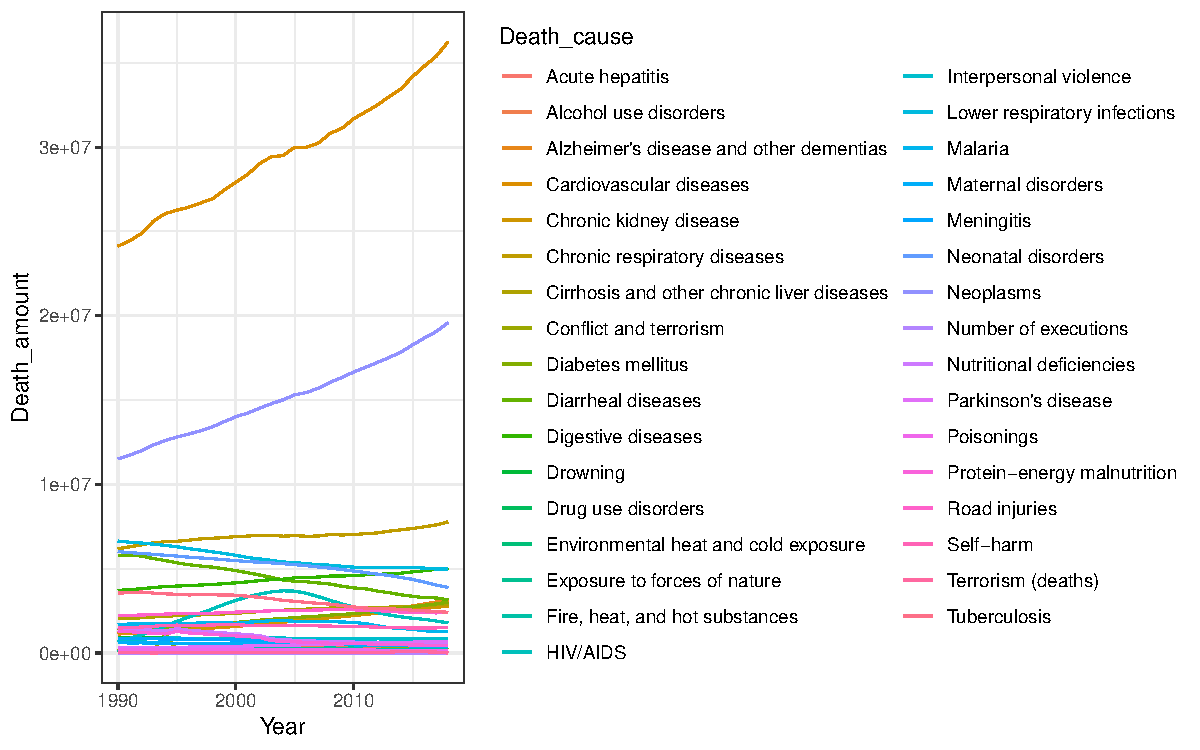
\includegraphics{Assignment4_files/figure-latex/worldplot-1.pdf}
\caption{\label{fig:worldplot}Number of deaths by cause, World, 1990 to 2019}
\end{figure}

\clearpage

\hypertarget{main-body}{%
\subsection{Main body}\label{main-body}}

\hypertarget{australia-and-switzerland}{%
\subsubsection{Australia and Switzerland}\label{australia-and-switzerland}}

\textbf{Q1: What can be observed in the chart of causes of death due to disease?}

\textbf{Q2: What can be observed in the chart of causes of death due to others?}

\textbf{(1).Plot death due to disease factors}

\begin{figure}
\centering
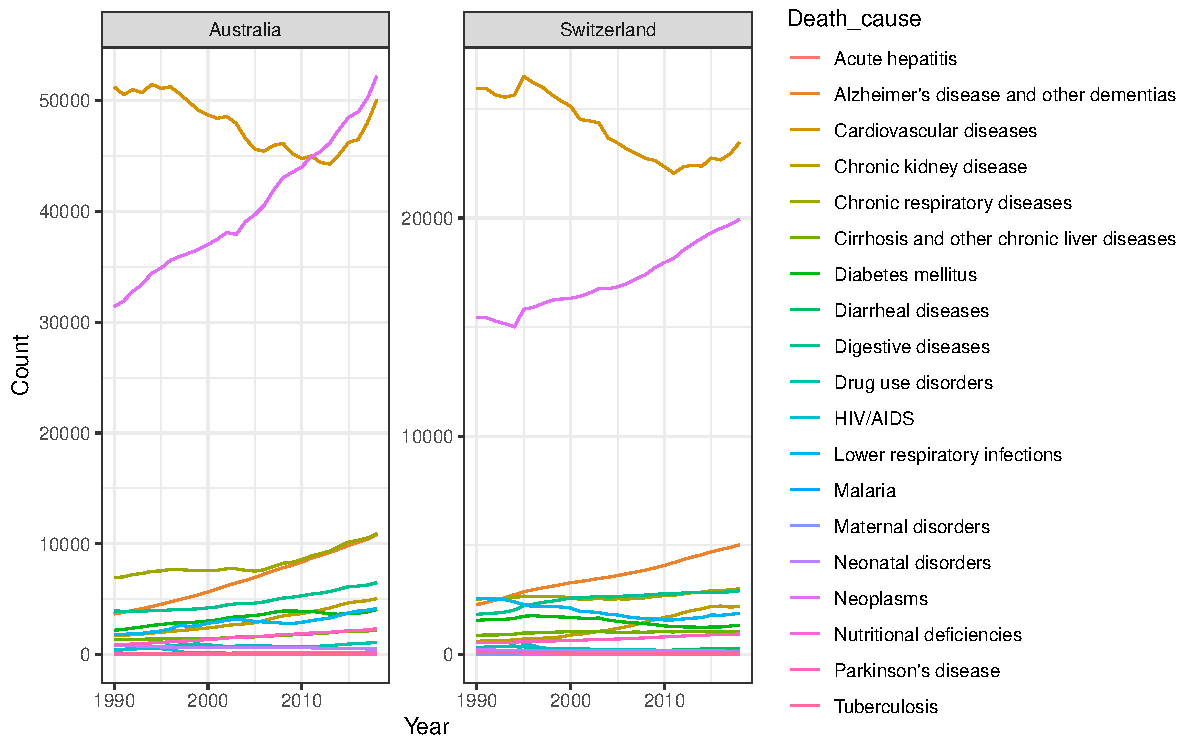
\includegraphics{Assignment4_files/figure-latex/diseaseplot-1.pdf}
\caption{\label{fig:diseaseplot}Number of deaths by disease causes, 1990 to 2018}
\end{figure}

As we can see from this graph\ref{fig:diseaseplot}, cardiovascular disease and Neoplasm are the leading causes of death in both Australia and Switzerland, with cardiovascular disease decreasing but starting to rise again after about 2011, and the number of deaths from Alzheimer's and neoplasm rising sharply.

This result confused me. I would have thought that because of the advancement of medicine, the causes of death from disease should gradually decrease.So I looked up these three conditions online, all of which are highly prevalent in older people, and then in this table \ref{tab:lifeexpendcy}, I listed life expectancy in Australia and Switzerland from 1990 to 2019.As can be seen from the table\ref{tab:lifeexpendcy}, life expectancy increases as the years go by, meaning that more people are living old enough so that the number of people who are sick increases.

\begin{table}

\caption{\label{tab:lifeexpendcy}Life Expectancy in Australia and Switzerland}
\centering
\begin{tabular}[t]{l|r|r}
\hline
Country & Year & Life\_expectancy\\
\hline
Australia & 1990 & 76.933\\
\hline
Australia & 1991 & 77.223\\
\hline
Australia & 1992 & 77.505\\
\hline
Australia & 1993 & 77.772\\
\hline
Australia & 1994 & 78.024\\
\hline
Australia & 1995 & 78.267\\
\hline
\end{tabular}
\end{table}

In plot\ref{fig:diseaseplot1}, I have added this life expectancy line to the first graph for better visualisation and you can see that it is all on an up trend.

\begin{figure}
\centering
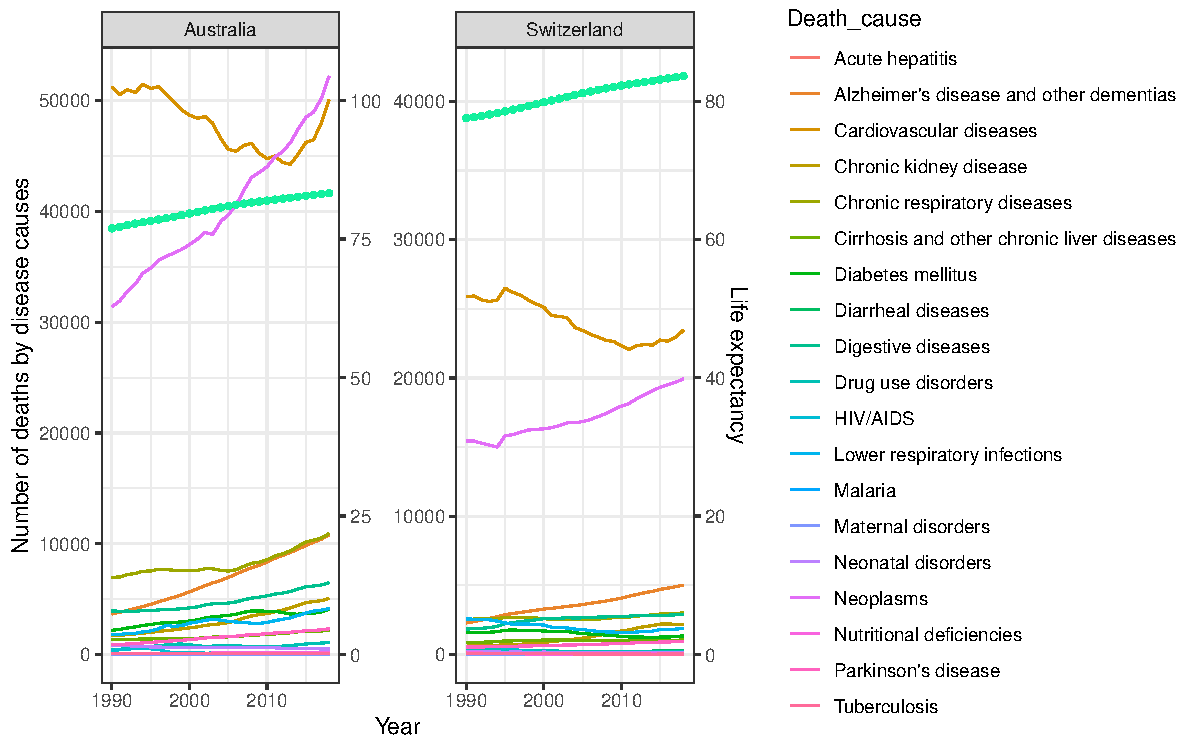
\includegraphics{Assignment4_files/figure-latex/diseaseplot1-1.pdf}
\caption{\label{fig:diseaseplot1}Add the line of life expectancy to fig1.}
\end{figure}

\textbf{(2).Plot death due to other factors}

\begin{figure}
\centering
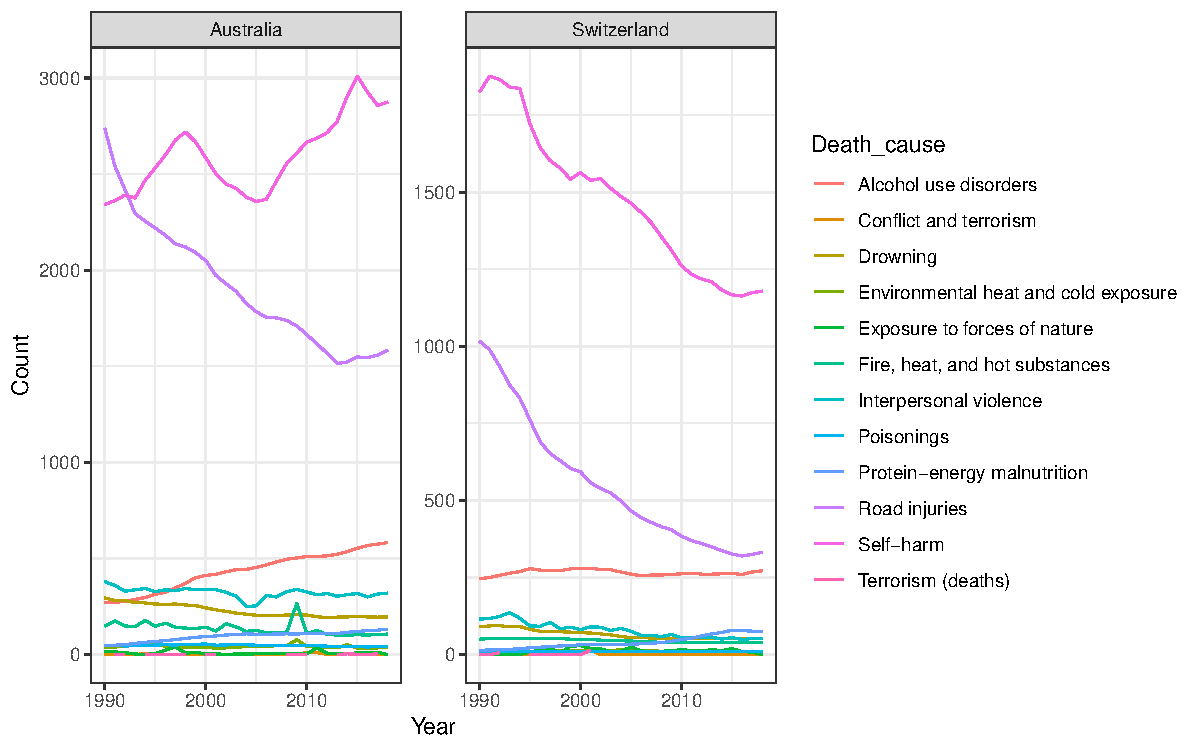
\includegraphics{Assignment4_files/figure-latex/otherplot-1.pdf}
\caption{\label{fig:otherplot}Number of deaths by other causes in Australia and Switzerland.}
\end{figure}

For other causes. This graph \ref{fig:otherplot}shows that self-harm, road injuries are the main causes of death from other causes. Road injuries have been decreasing and I think this is closely related to the improving traffic laws and the popularity of driving tests. I noticed that Australia had an unusual peak in 2009. I searched Google for three keywords: Australia Fire 2009 and I got the information that there was a very serious forest fire in Vic in 2009. \textcite{Bushfire} said that the Black Saturday fires started on 7 February 2009. Approximately 400 fires were recorded across Victoria, affecting 78 communities. A total of 173 people died in the fires, and 2029 houses were lost. So in 2009 an unusually high number of people died in fires in Australia.

In order to read data used R package \textcite{readr}, clean the data used R package \textcite{tidyverse}, plotting picture used R package \textcite{ggplot2}.

\clearpage

\hypertarget{china-and-india}{%
\section{China and India}\label{china-and-india}}

The health conditions are different due to the resources that different countries control. Which leads to an inequality in health in different areas \textcite{emadi2021global}. Countries in different developing conditions would have different health conditions. This section will focus on 2 typical developing countries : China and India. Investigate diseases that cause the most death in China and India, and how they are related with the GDP per capita.

\hypertarget{research-question}{%
\subsection{Research Question:}\label{research-question}}

\textbf{Q1: What are the diseases that cause the most death in China and India?}

\textbf{Q2: How the death caused by those diseases change with the change of GDP per capita?}

We will focusing on 6 typical diseases: they are : Cardiovascular Diseases, Diabetes mellitus, HIV, Neoplasms, Nutritional deficiencies and, Malaria

\begin{figure}
\centering
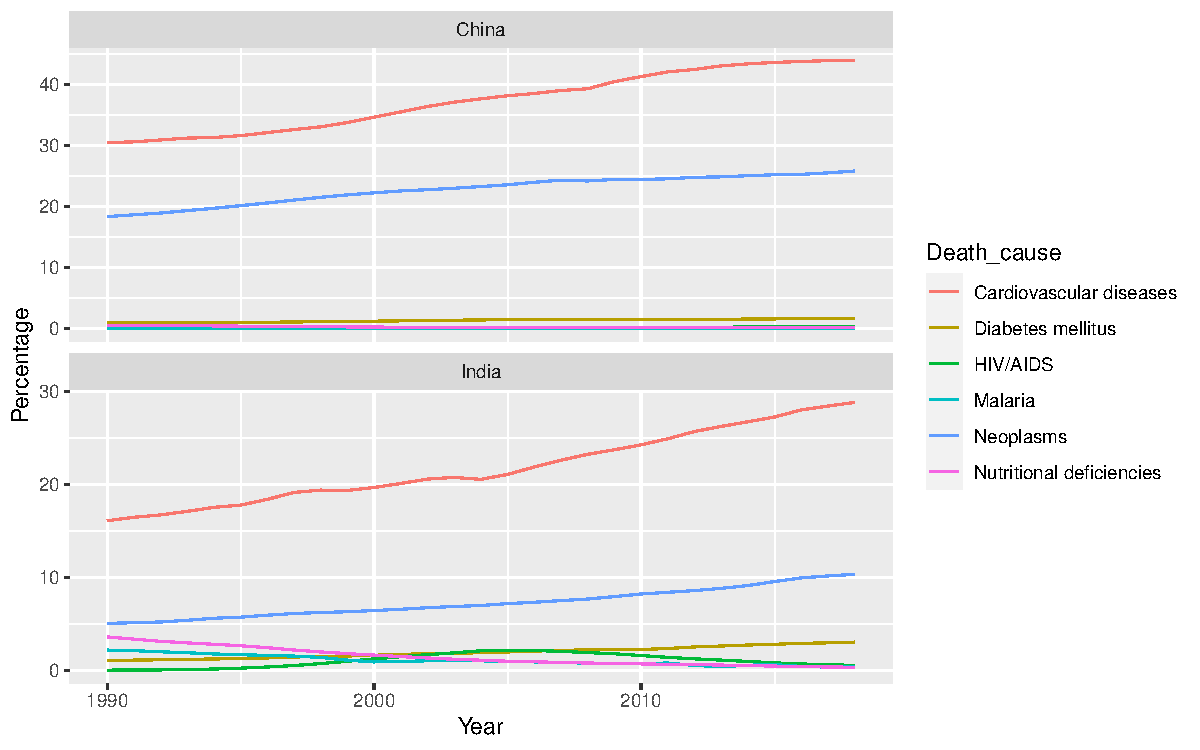
\includegraphics{Assignment4_files/figure-latex/percendeath-1.pdf}
\caption{\label{fig:percendeath}Percentage of different causes of death by year}
\end{figure}

In this graph \ref{fig:percendeath} , it is clear that both Cardiovascular Diseases and Neoplasms contribute the most among other diseases we are interested in both China and India and the trend is still increasing. So we will mainly focus on these 2 diseases. There are 43\% deaths caused by Cardiovascular diseases and 26\% caused by Neoplasms in China. 29\% deaths caused by Cardiovascular diseases and 10\% caused by Neoplasms in India. So, diseases that cause the most deaths in China and India are Cardiovascular diseases and Neoplasms.

\begin{figure}
\centering
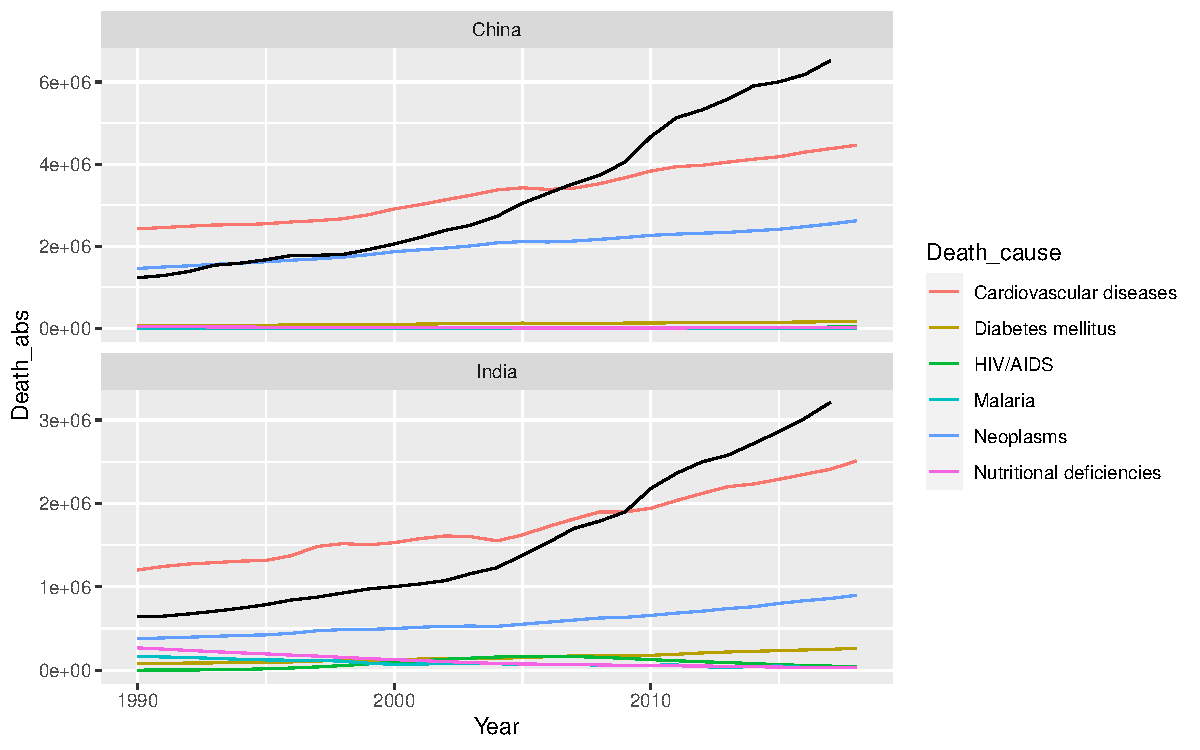
\includegraphics{Assignment4_files/figure-latex/totaldeath-1.pdf}
\caption{\label{fig:totaldeath}Total number of death by year and GDP per capita}
\end{figure}

In this graph \ref{fig:totaldeath}, we combine them with the GDP per capita graph, which is the black line. There is a clear trend that the death caused by these 2 diseases are highly correlated with GDP per capita. To find out the relations between them.

\begin{table}

\caption{\label{tab:modelparameter}Parameters of model}
\centering
\begin{tabular}[t]{l|l|r|r|r}
\hline
Country & Death\_cause & r.squared & intercept & slope\\
\hline
China & Cardiovascular diseases & 0.96 & 2085613.4 & 181.99\\
\hline
China & Neoplasms & 0.90 & 1404129.3 & 90.30\\
\hline
India & Cardiovascular diseases & 0.98 & 1031131.3 & 221.18\\
\hline
India & Neoplasms & 0.98 & 306150.6 & 85.49\\
\hline
\end{tabular}
\end{table}

I run a regression, using the death caused by ``Cardiovascular diseases'' and ``Neoplasms'' against GDP per capita showan in the table \ref{tab:modelparameter}. The r\^{}2 is quite high means they fitted into the linear model quite well

More than 90\% of deaths caused by Cardiovascular diseases and Neoplasms can be explained by the model. In China, for every 1 unit increase in the GDP per capita, the deaths caused by Cardiovascular diseases and Neoplasms will increase for 182 and 90. In India, for 1 unit increase in the GDP per capita, the deaths caused by Cardiovascular diseases and Neoplasms increased by 221 and 85 respectively.

It is corresponding to common sense as well. Because both Cardiovascular Diseases and Neoplasms occur more in the area with higher income. The longer one lives, the higher the possibility one can get these 2 diseases. Richer a country is, more resources can be used on transmitted diseases. therefore we can observe that death caused by transmitted diseases decreased to a very low level

In this part, I used package readr \textcite{readr} to read data, package broom \textcite{broom} to get statistic data from model, package knitr \textcite{knitr} to make table, package tidyverse \textcite{tidyverse} for basic calculation and package ggplot2 \textcite{ggplot2} to plot.

\printbibliography

\end{document}
